\documentclass[../fem.tex]{subfile}

\begin{document}
\section{Mesh Generation}%
\label{sec:mesh_generation}

For the implementation of finite element methods, it is required to first
discretize the global domain into a set of finite subdomains. Each subdomain is
called an element. It is then possible to compute the values of the local
system of equations with respect to a given element, then to combine these
values to construct the global system. The first step is to discretize the
global domain into a set of finite elements.

These elements can be of the form of a $N$ sided polygon, not that it will not
be regular each side will have different lengths. This paper will utilize
triangular meshes, but many implementations also implement quadrangle and
hexagonal meshes. Since the construction of meshes with elements with more than
three sides is considerably more difficult, we will limit this paper to only
discussing the triangular mesh construction.

Constructing the triangular mesh is the most generalized method, as any polygon
with more edges can be constructed by several triangles. Thus the mesh of
polygons with more than three sides can be derived from the triangular mesh,
without significant difficulty.

The process that will be used for the construction of the triangular mesh is
knows as Constrained Delaunay Triangulation. Then to improve the mesh and
consequently improve the accuracy of the approximation, a mesh refinement
algorithm is utilized to ensure that the elements of the mesh are of an
acceptable quality.

\subsection{Delaunay Triangulation}%
\label{sub:delaunay_triangulation}

Delaunay triangulation is the straight line dual of the Voronoi diagram. The
Delaunay triangulation of a domain is commonly used in many different
situations, including for the purpose of mesh generation for finite element
analysis.

The key property of Delaunay triangulation is that no point may lie within the
circumcircle of any other triangle.

\begin{definition}[Circumcircle]
  The circumcircle of a triangle is the circle is defined by having all three
  vertices of the triangle on the circle. For any given triangle there is only
  one such circle that satisfies this. In figure \ref{fig:circumcircle}, a
  depiction of the circumcircle for a provided triangle is given.
\end{definition}

\begin{definition}[Delaunay Triangulation]
   Let $S$ be a set of points in the plane $\R^2$. A triangulation $T$ is a
   \textit{Delaunay Triangulation}($DT$) of $S$ if for each triangle $t$ of $T$
   there exists a circle $C$ with the following properties:
   \begin{enumerate}
     \item all of the vertices of the triangle $t$ are on the boundary of
       circle $C$,
       \begin{align*}
          p\in\partial C\quad\forall p\in t
       \end{align*}
     \item and no other vertex of $S$ is in the interior of $C$.
       \begin{align*}
         p\notin S\quad\forall p\in\text{Int}(C)
       \end{align*}
   \end{enumerate}
\end{definition}

\begin{figure}[htpb]
  \centering
  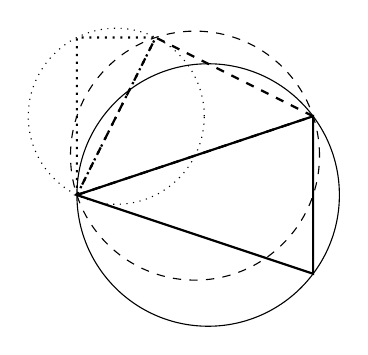
\begin{tikzpicture}[scale=1, transform shape]
\draw[solid,thick] (0,1) -- (3,0) -- (3,2) -- cycle;
\draw[solid] (1.667, 1) circle (1.66666);
\draw[dashed,thick] (0,1) -- (3,2) -- (1,3) -- cycle;
\draw[dashed] (1.5, 1.5) circle (1.58113);
\draw[dotted,thick] (0,1) -- (1,3) -- (0,3) -- cycle;
\draw[dotted] (0.5,2) circle (1.11803);
\end{tikzpicture}


  \caption{Demonstration of the circumcircle definition of Delaunay
  triangulation. This shows how the circumcircle of each triangle does not
contain any vertex from any other triangles.}
\label{fig:circumcircle}
\end{figure}

By this definition of the Delaunay triangulation, the triangulation is unique
for most sets of points $S$. The only exception to this rule is when a set of
four points construct the square. For the square, there are two equally valid
triangulations, and dependent on the implementation one or the other must be
selected.

A major advantage of the Delaunay triangulation for mesh generation is that it
inherently avoids triangles with small included angles, as the circumcircles of
these triangles would be very large, and would likely include other vertices.
This avoidance is extremely useful in finite element analysis and will produce
more accurate approximations of the solution to the partial differential
equation.

There are many different algorithms that can be implemented for the
construction of the Delaunay triangulation. The notable methods include; Divide
and Conquer, Incremental, Sweep Line, and Edge Flipping. The specifics of these
algorithms will be discussed further in section \ref{sec:mesh_generation2}.

With the Delaunay triangulation constructed, one must next apply the boundaries
of the domain to the mesh. The process is called the construction of the
Constrained Delaunay Triangulation.

\subsection{Constrained Delaunay Triangulation}%
\label{sub:constrained_delaunay_triangulation}

The Constrained Delaunay Triangulation, is a modification of the Delaunay
Triangulation such that specified edges and vertices are forced to exists in
the triangulation. Because of the forcing of edges into the triangulation, the
mesh may not strictly satisfy the definition of Delaunay triangulation. Thus we
define the constrained triangulation as the closest triangulation to the
Delaunay triangulation that includes all of the required edges.

This sense of ``closeness'' to the Delaunay mesh is such that we use as few
modifications from a Delaunay triangulation in order to enforce the constrained
edges to construct the constrained Delaunay triangulation.

The constrained edges are most commonly utilized for the purpose of defining
boundaries of the domain or enforcing a location of a medium change. Since the
result of the unconstrained Delaunay triangulation will have a strictly convex
shape. This makes it necessary to apply the edge constraints for all domains
that do not have a strictly convex outer hull.

There are a number of methods for the construction of the constrained Delaunay
triangulation. A few of these implementations enforce the constraints during
the initial construction of the triangulation. However, more commonly the
constraints are enforced upon an already constructed triangulation. The details
on the implementation of these algorithms are discussed in section
\ref{sec:mesh_generation2}.

\begin{figure}[htpb]
  \centering
  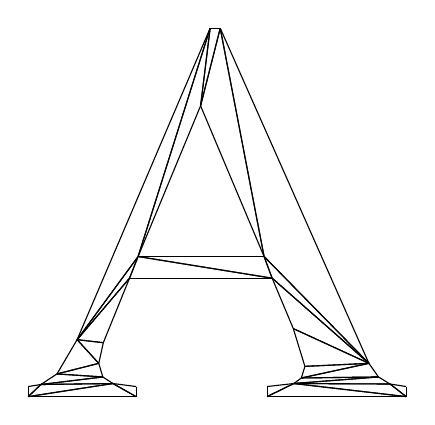
\begin{tikzpicture}[scale=8.0]
\draw (0.2,-0.7924) -- (0.22,-0.7732);
\draw (0.22,-0.7732) -- (0.2,-0.7764);
\draw (0.2,-0.7764) -- (0.2,-0.7924);
\draw (0.22,-0.7732) -- (0.2,-0.7924);
\draw (0.2,-0.7924) -- (0.3344,-0.7716);
\draw (0.3344,-0.7716) -- (0.22,-0.7732);
\draw (0.3712,-0.7924) -- (0.3712,-0.7764);
\draw (0.3712,-0.7764) -- (0.3344,-0.7716);
\draw (0.3344,-0.7716) -- (0.3712,-0.7924);
\draw (0.3344,-0.7716) -- (0.3184,-0.7612);
\draw (0.3184,-0.7612) -- (0.22,-0.7732);
\draw (0.22,-0.7732) -- (0.3344,-0.7716);
\draw (0.3712,-0.7924) -- (0.3344,-0.7716);
\draw (0.3344,-0.7716) -- (0.2,-0.7924);
\draw (0.2,-0.7924) -- (0.3712,-0.7924);
\draw (0.22,-0.7732) -- (0.3184,-0.7612);
\draw (0.3184,-0.7612) -- (0.2456,-0.7564);
\draw (0.2456,-0.7564) -- (0.22,-0.7732);
\draw (0.2456,-0.7564) -- (0.312,-0.7396);
\draw (0.312,-0.7396) -- (0.2776,-0.702);
\draw (0.2776,-0.702) -- (0.2456,-0.7564);
\draw (0.312,-0.7396) -- (0.2456,-0.7564);
\draw (0.2456,-0.7564) -- (0.3184,-0.7612);
\draw (0.3184,-0.7612) -- (0.312,-0.7396);
\draw (0.2776,-0.702) -- (0.312,-0.7396);
\draw (0.312,-0.7396) -- (0.3192,-0.7068);
\draw (0.3192,-0.7068) -- (0.2776,-0.702);
\draw (0.4888,-0.2076) -- (0.2776,-0.702);
\draw (0.2776,-0.702) -- (0.3744,-0.57);
\draw (0.3744,-0.57) -- (0.4888,-0.2076);
\draw (0.3608,-0.6044) -- (0.3744,-0.57);
\draw (0.3744,-0.57) -- (0.2776,-0.702);
\draw (0.2776,-0.702) -- (0.3608,-0.6044);
\draw (0.3744,-0.57) -- (0.3608,-0.6044);
\draw (0.3608,-0.6044) -- (0.5872,-0.6044);
\draw (0.5872,-0.6044) -- (0.3744,-0.57);
\draw (0.3608,-0.6044) -- (0.2776,-0.702);
\draw (0.2776,-0.702) -- (0.3192,-0.7068);
\draw (0.3192,-0.7068) -- (0.3608,-0.6044);
\draw (0.4888,-0.2076) -- (0.3744,-0.57);
\draw (0.3744,-0.57) -- (0.4736,-0.3308);
\draw (0.4736,-0.3308) -- (0.4888,-0.2076);
\draw (0.5792,-0.7924) -- (0.6216,-0.7716);
\draw (0.6216,-0.7716) -- (0.5792,-0.7764);
\draw (0.5792,-0.7764) -- (0.5792,-0.7924);
\draw (0.6216,-0.7716) -- (0.5792,-0.7924);
\draw (0.5792,-0.7924) -- (0.8,-0.7924);
\draw (0.8,-0.7924) -- (0.6216,-0.7716);
\draw (0.8,-0.7924) -- (0.8,-0.7764);
\draw (0.8,-0.7764) -- (0.7744,-0.7724);
\draw (0.7744,-0.7724) -- (0.8,-0.7924);
\draw (0.756,-0.7612) -- (0.6216,-0.7716);
\draw (0.6216,-0.7716) -- (0.7744,-0.7724);
\draw (0.7744,-0.7724) -- (0.756,-0.7612);
\draw (0.756,-0.7612) -- (0.6336,-0.7628);
\draw (0.6336,-0.7628) -- (0.6216,-0.7716);
\draw (0.6216,-0.7716) -- (0.756,-0.7612);
\draw (0.7744,-0.7724) -- (0.6216,-0.7716);
\draw (0.6216,-0.7716) -- (0.8,-0.7924);
\draw (0.8,-0.7924) -- (0.7744,-0.7724);
\draw (0.5048,-0.2076) -- (0.5744,-0.57);
\draw (0.5744,-0.57) -- (0.7408,-0.7396);
\draw (0.7408,-0.7396) -- (0.5048,-0.2076);
\draw (0.3744,-0.57) -- (0.5872,-0.6044);
\draw (0.5872,-0.6044) -- (0.5744,-0.57);
\draw (0.5744,-0.57) -- (0.3744,-0.57);
\draw (0.4888,-0.2076) -- (0.4736,-0.3308);
\draw (0.4736,-0.3308) -- (0.5048,-0.2076);
\draw (0.5048,-0.2076) -- (0.4888,-0.2076);
\draw (0.5744,-0.57) -- (0.5872,-0.6044);
\draw (0.5872,-0.6044) -- (0.7408,-0.7396);
\draw (0.7408,-0.7396) -- (0.5744,-0.57);
\draw (0.4736,-0.3308) -- (0.5744,-0.57);
\draw (0.5744,-0.57) -- (0.5048,-0.2076);
\draw (0.5048,-0.2076) -- (0.4736,-0.3308);
\draw (0.6336,-0.7628) -- (0.7408,-0.7396);
\draw (0.7408,-0.7396) -- (0.6392,-0.7444);
\draw (0.6392,-0.7444) -- (0.6336,-0.7628);
\draw (0.7408,-0.7396) -- (0.6336,-0.7628);
\draw (0.6336,-0.7628) -- (0.756,-0.7612);
\draw (0.756,-0.7612) -- (0.7408,-0.7396);
\draw (0.6208,-0.6844) -- (0.7408,-0.7396);
\draw (0.7408,-0.7396) -- (0.5872,-0.6044);
\draw (0.5872,-0.6044) -- (0.6208,-0.6844);
\draw (0.7408,-0.7396) -- (0.6208,-0.6844);
\draw (0.6208,-0.6844) -- (0.6392,-0.7444);
\draw (0.6392,-0.7444) -- (0.7408,-0.7396);
\end{tikzpicture}

  \caption{Constrained Delaunay triaangulation of the letter $A$. This mesh has
  been constructed without any quality or area refinements.}
  \label{fig:delaunay_constrained}
\end{figure}

\subsection{Mesh Refinement}%
\label{sub:mesh_refinement}

The direct output of the constrained Delaunay triangulation algorithms may be
sufficient in a few situations, but for most cases, it would result in
suboptimal meshes. For generalizability, we discuss the methods that are utilized
to refine the generated mesh, thus improving the quality of the meshes.

Mesh refinement is almost always required, because, along constrained edges,
there may only be a single element. This element is forced to have one of its
edges to be the entity of the constrained edge. This tends to lead to skinny
triangles, ones whos minimum interior angle is very small. There are frequently
undesirable in the final mesh. We denote that these triangles are not
\textit{well-shaped}.

\begin{definition}[Well-Shaped] \label{def:well_shaped}
  A triangle is well-shaped if all its interior angles are greater than or
  equal to some defined constant angle $\alpha$ (commonly
  $\alpha\approx30^\circ$).
\end{definition}

It is also possible that all the elements in the mesh are well-shaped, but they
could all be very large. A finer mesh will always result in more accurate
approximations, as will be made clear later. Thus we may also want to define a
notion of \textit{well-sized} triangles so that it is possible to refine the
element size in the mesh.

\begin{definition}[Well-Sized] \label{def:well_sized}
  A triangle is well-sized if the area of the triangle satisfies some user-defined grading function $g$ (commonly $g=\text{const}$). This function can
  use any criteria for determining if a triangle satisfies it, as long as there
  exists a value $\delta>0$ such that any well-shaped triangle that fits within
  a circle of radius $\delta$ would satisfy the grading function.
\end{definition}

This definition of the well-sized triangles describes that any function can be
used in order to define when a triangle is well-sized. This is very important
in constructing meshes that are very fine around specified features, and the
coarser in the unimportant regions. The one restriction of the grading function
is that there must be some lower bound, such that all triangles that fit within
the lower bound will be accepted. This enforces that the grading function may
not require triangles to become infinitely small.

We will now define what it means for a triangle to be ``nice''.

\begin{definition}[nice] \label{def:nice_tri}
  A triangle is said to be \textit{nice}, if it is both well-shaped (Def
  \ref{def:well_shaped}) and well-sized (Def \ref{def:well_sized}).
\end{definition}

Using these definitions for how to classify the elements of a mesh, it becomes
possible to implement algorithms in order to refine any mesh. The
technicalities of the mesh refinement algorithms are discussed in
\ref{sub:mesh_refinement2}.

\begin{figure}[htpb]
  \centering
     \begin{minipage}{0.4\textwidth}
     \begin{center}
       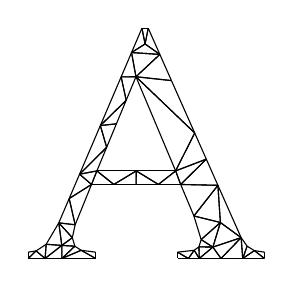
\begin{tikzpicture}[scale=5]
\draw (0.2,-0.7924) -- (0.22,-0.7732);
\draw (0.22,-0.7732) -- (0.2,-0.7764);
\draw (0.2,-0.7764) -- (0.2,-0.7924);
\draw (0.28531162790697684,-0.7592558139534884) -- (0.2428,-0.7924);
\draw (0.2428,-0.7924) -- (0.28559999999999997,-0.7924);
\draw (0.28559999999999997,-0.7924) -- (0.28531162790697684,-0.7592558139534884);
\draw (0.4736,-0.3308) -- (0.5343,-0.2741);
\draw (0.5343,-0.2741) -- (0.46240000000000003,-0.2694);
\draw (0.46240000000000003,-0.2694) -- (0.4736,-0.3308);
\draw (0.4174,-0.6044) -- (0.47400000000000003,-0.6044);
\draw (0.47400000000000003,-0.6044) -- (0.47440000000000004,-0.57);
\draw (0.47440000000000004,-0.57) -- (0.4174,-0.6044);
\draw (0.3712,-0.7924) -- (0.3712,-0.7764);
\draw (0.3712,-0.7764) -- (0.3344,-0.7716);
\draw (0.3344,-0.7716) -- (0.3712,-0.7924);
\draw (0.6216,-0.7716) -- (0.6068,-0.7924);
\draw (0.6068,-0.7924) -- (0.6344000000000001,-0.7924);
\draw (0.6344000000000001,-0.7924) -- (0.6216,-0.7716);
\draw (0.436,-0.3312) -- (0.44880000000000003,-0.39059999999999995);
\draw (0.44880000000000003,-0.39059999999999995) -- (0.4736,-0.3308);
\draw (0.4736,-0.3308) -- (0.436,-0.3312);
\draw (0.3184,-0.7612) -- (0.312,-0.7396);
\draw (0.312,-0.7396) -- (0.28531162790697684,-0.7592558139534884);
\draw (0.28531162790697684,-0.7592558139534884) -- (0.3184,-0.7612);
\draw (0.28559999999999997,-0.7924) -- (0.3344,-0.7716);
\draw (0.3344,-0.7716) -- (0.3184,-0.7612);
\draw (0.3184,-0.7612) -- (0.28559999999999997,-0.7924);
\draw (0.3712,-0.7924) -- (0.3344,-0.7716);
\draw (0.3344,-0.7716) -- (0.28559999999999997,-0.7924);
\draw (0.28559999999999997,-0.7924) -- (0.3712,-0.7924);
\draw (0.3744,-0.57) -- (0.3608,-0.6044);
\draw (0.3608,-0.6044) -- (0.4174,-0.6044);
\draw (0.4174,-0.6044) -- (0.3744,-0.57);
\draw (0.2456,-0.7564) -- (0.22,-0.7732);
\draw (0.22,-0.7732) -- (0.2428,-0.7924);
\draw (0.2428,-0.7924) -- (0.2456,-0.7564);
\draw (0.28531162790697684,-0.7592558139534884) -- (0.2776,-0.702);
\draw (0.2776,-0.702) -- (0.2456,-0.7564);
\draw (0.2456,-0.7564) -- (0.28531162790697684,-0.7592558139534884);
\draw (0.28559999999999997,-0.7924) -- (0.3184,-0.7612);
\draw (0.3184,-0.7612) -- (0.28531162790697684,-0.7592558139534884);
\draw (0.28531162790697684,-0.7592558139534884) -- (0.28559999999999997,-0.7924);
\draw (0.2776,-0.702) -- (0.312,-0.7396);
\draw (0.312,-0.7396) -- (0.3192,-0.7068);
\draw (0.3192,-0.7068) -- (0.2776,-0.702);
\draw (0.3192,-0.7068) -- (0.304,-0.6402);
\draw (0.304,-0.6402) -- (0.2776,-0.702);
\draw (0.2776,-0.702) -- (0.3192,-0.7068);
\draw (0.3744,-0.57) -- (0.33039999999999997,-0.5784);
\draw (0.33039999999999997,-0.5784) -- (0.3608,-0.6044);
\draw (0.3608,-0.6044) -- (0.3744,-0.57);
\draw (0.6208,-0.6844) -- (0.6818,-0.6066);
\draw (0.6818,-0.6066) -- (0.5872,-0.6044);
\draw (0.5872,-0.6044) -- (0.6208,-0.6844);
\draw (0.3992,-0.5102) -- (0.33039999999999997,-0.5784);
\draw (0.33039999999999997,-0.5784) -- (0.3744,-0.57);
\draw (0.3744,-0.57) -- (0.3992,-0.5102);
\draw (0.5306000000000001,-0.6044) -- (0.5872,-0.6044);
\draw (0.5872,-0.6044) -- (0.5744,-0.57);
\draw (0.5744,-0.57) -- (0.5306000000000001,-0.6044);
\draw (0.304,-0.6402) -- (0.3192,-0.7068);
\draw (0.3192,-0.7068) -- (0.3608,-0.6044);
\draw (0.3608,-0.6044) -- (0.304,-0.6402);
\draw (0.2776,-0.702) -- (0.28531162790697684,-0.7592558139534884);
\draw (0.28531162790697684,-0.7592558139534884) -- (0.312,-0.7396);
\draw (0.312,-0.7396) -- (0.2776,-0.702);
\draw (0.6880643863623271,-0.7010295113359224) -- (0.6690356340288925,-0.7635325842696628);
\draw (0.6690356340288925,-0.7635325842696628) -- (0.7408,-0.7396);
\draw (0.7408,-0.7396) -- (0.6880643863623271,-0.7010295113359224);
\draw (0.22,-0.7732) -- (0.2,-0.7924);
\draw (0.2,-0.7924) -- (0.2428,-0.7924);
\draw (0.2428,-0.7924) -- (0.22,-0.7732);
\draw (0.44880000000000003,-0.39059999999999995) -- (0.3832,-0.4548);
\draw (0.3832,-0.4548) -- (0.42400000000000004,-0.45039999999999997);
\draw (0.42400000000000004,-0.45039999999999997) -- (0.44880000000000003,-0.39059999999999995);
\draw (0.6068,-0.7924) -- (0.5792,-0.7764);
\draw (0.5792,-0.7764) -- (0.5792,-0.7924);
\draw (0.5792,-0.7924) -- (0.6068,-0.7924);
\draw (0.7448,-0.7924) -- (0.8,-0.7924);
\draw (0.8,-0.7924) -- (0.7744,-0.7724);
\draw (0.7744,-0.7724) -- (0.7448,-0.7924);
\draw (0.3832,-0.4548) -- (0.3992,-0.5102);
\draw (0.3992,-0.5102) -- (0.42400000000000004,-0.45039999999999997);
\draw (0.42400000000000004,-0.45039999999999997) -- (0.3832,-0.4548);
\draw (0.4736,-0.3308) -- (0.6228,-0.4736);
\draw (0.6228,-0.4736) -- (0.5638000000000001,-0.3406);
\draw (0.5638000000000001,-0.3406) -- (0.4736,-0.3308);
\draw (0.8,-0.7924) -- (0.8,-0.7764);
\draw (0.8,-0.7764) -- (0.7744,-0.7724);
\draw (0.7744,-0.7724) -- (0.8,-0.7924);
\draw (0.6523,-0.5401) -- (0.6228,-0.4736);
\draw (0.6228,-0.4736) -- (0.5744,-0.57);
\draw (0.5744,-0.57) -- (0.6523,-0.5401);
\draw (0.7408,-0.7396) -- (0.6896,-0.7924);
\draw (0.6896,-0.7924) -- (0.7448,-0.7924);
\draw (0.7448,-0.7924) -- (0.7408,-0.7396);
\draw (0.6216,-0.7716) -- (0.6344000000000001,-0.7924);
\draw (0.6344000000000001,-0.7924) -- (0.6336,-0.7628);
\draw (0.6336,-0.7628) -- (0.6216,-0.7716);
\draw (0.756,-0.7612) -- (0.7448,-0.7924);
\draw (0.7448,-0.7924) -- (0.7744,-0.7724);
\draw (0.7744,-0.7724) -- (0.756,-0.7612);
\draw (0.756,-0.7612) -- (0.7408,-0.7396);
\draw (0.7408,-0.7396) -- (0.7448,-0.7924);
\draw (0.7448,-0.7924) -- (0.756,-0.7612);
\draw (0.5872,-0.6044) -- (0.6523,-0.5401);
\draw (0.6523,-0.5401) -- (0.5744,-0.57);
\draw (0.5744,-0.57) -- (0.5872,-0.6044);
\draw (0.6896,-0.7924) -- (0.6690356340288925,-0.7635325842696628);
\draw (0.6690356340288925,-0.7635325842696628) -- (0.6344000000000001,-0.7924);
\draw (0.6344000000000001,-0.7924) -- (0.6896,-0.7924);
\draw (0.5343,-0.2741) -- (0.4736,-0.3308);
\draw (0.4736,-0.3308) -- (0.5638000000000001,-0.3406);
\draw (0.5638000000000001,-0.3406) -- (0.5343,-0.2741);
\draw (0.47440000000000004,-0.57) -- (0.3744,-0.57);
\draw (0.3744,-0.57) -- (0.4174,-0.6044);
\draw (0.4174,-0.6044) -- (0.47440000000000004,-0.57);
\draw (0.7408,-0.7396) -- (0.6818,-0.6066);
\draw (0.6818,-0.6066) -- (0.6880643863623271,-0.7010295113359224);
\draw (0.6880643863623271,-0.7010295113359224) -- (0.7408,-0.7396);
\draw (0.4736,-0.3308) -- (0.46240000000000003,-0.2694);
\draw (0.46240000000000003,-0.2694) -- (0.436,-0.3312);
\draw (0.436,-0.3312) -- (0.4736,-0.3308);
\draw (0.5872,-0.6044) -- (0.6818,-0.6066);
\draw (0.6818,-0.6066) -- (0.6523,-0.5401);
\draw (0.6523,-0.5401) -- (0.5872,-0.6044);
\draw (0.5744,-0.57) -- (0.6228,-0.4736);
\draw (0.6228,-0.4736) -- (0.4736,-0.3308);
\draw (0.4736,-0.3308) -- (0.5744,-0.57);
\draw (0.6336,-0.7628) -- (0.6344000000000001,-0.7924);
\draw (0.6344000000000001,-0.7924) -- (0.6690356340288925,-0.7635325842696628);
\draw (0.6690356340288925,-0.7635325842696628) -- (0.6336,-0.7628);
\draw (0.6690356340288925,-0.7635325842696628) -- (0.6392,-0.7444);
\draw (0.6392,-0.7444) -- (0.6336,-0.7628);
\draw (0.6336,-0.7628) -- (0.6690356340288925,-0.7635325842696628);
\draw (0.6880643863623271,-0.7010295113359224) -- (0.6208,-0.6844);
\draw (0.6208,-0.6844) -- (0.6392,-0.7444);
\draw (0.6392,-0.7444) -- (0.6880643863623271,-0.7010295113359224);
\draw (0.6392,-0.7444) -- (0.6690356340288925,-0.7635325842696628);
\draw (0.6690356340288925,-0.7635325842696628) -- (0.6880643863623271,-0.7010295113359224);
\draw (0.6880643863623271,-0.7010295113359224) -- (0.6392,-0.7444);
\draw (0.5792,-0.7764) -- (0.6068,-0.7924);
\draw (0.6068,-0.7924) -- (0.6216,-0.7716);
\draw (0.6216,-0.7716) -- (0.5792,-0.7764);
\draw (0.4968,-0.24755631067961165) -- (0.4888,-0.2076);
\draw (0.4888,-0.2076) -- (0.46240000000000003,-0.2694);
\draw (0.46240000000000003,-0.2694) -- (0.4968,-0.24755631067961165);
\draw (0.46240000000000003,-0.2694) -- (0.5343,-0.2741);
\draw (0.5343,-0.2741) -- (0.4968,-0.24755631067961165);
\draw (0.4968,-0.24755631067961165) -- (0.46240000000000003,-0.2694);
\draw (0.2428,-0.7924) -- (0.28531162790697684,-0.7592558139534884);
\draw (0.28531162790697684,-0.7592558139534884) -- (0.2456,-0.7564);
\draw (0.2456,-0.7564) -- (0.2428,-0.7924);
\draw (0.6818,-0.6066) -- (0.6208,-0.6844);
\draw (0.6208,-0.6844) -- (0.6880643863623271,-0.7010295113359224);
\draw (0.6880643863623271,-0.7010295113359224) -- (0.6818,-0.6066);
\draw (0.6896,-0.7924) -- (0.7408,-0.7396);
\draw (0.7408,-0.7396) -- (0.6690356340288925,-0.7635325842696628);
\draw (0.6690356340288925,-0.7635325842696628) -- (0.6896,-0.7924);
\draw (0.47440000000000004,-0.57) -- (0.5306000000000001,-0.6044);
\draw (0.5306000000000001,-0.6044) -- (0.5744,-0.57);
\draw (0.5744,-0.57) -- (0.47440000000000004,-0.57);
\draw (0.5306000000000001,-0.6044) -- (0.47440000000000004,-0.57);
\draw (0.47440000000000004,-0.57) -- (0.47400000000000003,-0.6044);
\draw (0.47400000000000003,-0.6044) -- (0.5306000000000001,-0.6044);
\draw (0.3832,-0.4548) -- (0.44880000000000003,-0.39059999999999995);
\draw (0.44880000000000003,-0.39059999999999995) -- (0.436,-0.3312);
\draw (0.436,-0.3312) -- (0.3832,-0.4548);
\draw (0.3608,-0.6044) -- (0.33039999999999997,-0.5784);
\draw (0.33039999999999997,-0.5784) -- (0.304,-0.6402);
\draw (0.304,-0.6402) -- (0.3608,-0.6044);
\draw (0.33039999999999997,-0.5784) -- (0.3992,-0.5102);
\draw (0.3992,-0.5102) -- (0.3832,-0.4548);
\draw (0.3832,-0.4548) -- (0.33039999999999997,-0.5784);
\draw (0.5048,-0.2076) -- (0.4888,-0.2076);
\draw (0.4888,-0.2076) -- (0.4968,-0.24755631067961165);
\draw (0.4968,-0.24755631067961165) -- (0.5048,-0.2076);
\draw (0.5343,-0.2741) -- (0.5048,-0.2076);
\draw (0.5048,-0.2076) -- (0.4968,-0.24755631067961165);
\draw (0.4968,-0.24755631067961165) -- (0.5343,-0.2741);
\end{tikzpicture}

       (a)
     \end{center}
   \end{minipage}
   \begin{minipage}{0.4\textwidth}
     \begin{center}
       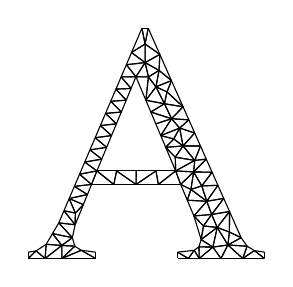
\begin{tikzpicture}[scale=5]
\draw (0.2,-0.7924) -- (0.22,-0.7732);
\draw (0.22,-0.7732) -- (0.2,-0.7764);
\draw (0.2,-0.7764) -- (0.2,-0.7924);
\draw (0.28531162790697684,-0.7592558139534884) -- (0.2428,-0.7924);
\draw (0.2428,-0.7924) -- (0.28559999999999997,-0.7924);
\draw (0.28559999999999997,-0.7924) -- (0.28531162790697684,-0.7592558139534884);
\draw (0.4968406949074053,-0.2948391566292681) -- (0.46240000000000003,-0.2694);
\draw (0.46240000000000003,-0.2694) -- (0.4492,-0.3003);
\draw (0.4492,-0.3003) -- (0.4968406949074053,-0.2948391566292681);
\draw (0.47400000000000003,-0.6044) -- (0.47440000000000004,-0.57);
\draw (0.47440000000000004,-0.57) -- (0.4244,-0.57);
\draw (0.4244,-0.57) -- (0.47400000000000003,-0.6044);
\draw (0.3712,-0.7924) -- (0.3712,-0.7764);
\draw (0.3712,-0.7764) -- (0.3344,-0.7716);
\draw (0.3344,-0.7716) -- (0.3712,-0.7924);
\draw (0.6216,-0.7716) -- (0.6068,-0.7924);
\draw (0.6068,-0.7924) -- (0.6344000000000001,-0.7924);
\draw (0.6344000000000001,-0.7924) -- (0.6216,-0.7716);
\draw (0.436,-0.3312) -- (0.46120000000000005,-0.36069999999999997);
\draw (0.46120000000000005,-0.36069999999999997) -- (0.4736,-0.3308);
\draw (0.4736,-0.3308) -- (0.436,-0.3312);
\draw (0.3184,-0.7612) -- (0.312,-0.7396);
\draw (0.312,-0.7396) -- (0.28531162790697684,-0.7592558139534884);
\draw (0.28531162790697684,-0.7592558139534884) -- (0.3184,-0.7612);
\draw (0.28559999999999997,-0.7924) -- (0.3344,-0.7716);
\draw (0.3344,-0.7716) -- (0.3184,-0.7612);
\draw (0.3184,-0.7612) -- (0.28559999999999997,-0.7924);
\draw (0.3712,-0.7924) -- (0.3344,-0.7716);
\draw (0.3344,-0.7716) -- (0.28559999999999997,-0.7924);
\draw (0.28559999999999997,-0.7924) -- (0.3712,-0.7924);
\draw (0.3744,-0.57) -- (0.3608,-0.6044);
\draw (0.3608,-0.6044) -- (0.4174,-0.6044);
\draw (0.4174,-0.6044) -- (0.3744,-0.57);
\draw (0.2456,-0.7564) -- (0.22,-0.7732);
\draw (0.22,-0.7732) -- (0.2428,-0.7924);
\draw (0.2428,-0.7924) -- (0.2456,-0.7564);
\draw (0.28531162790697684,-0.7592558139534884) -- (0.2616,-0.7292);
\draw (0.2616,-0.7292) -- (0.2456,-0.7564);
\draw (0.2456,-0.7564) -- (0.28531162790697684,-0.7592558139534884);
\draw (0.28559999999999997,-0.7924) -- (0.3184,-0.7612);
\draw (0.3184,-0.7612) -- (0.28531162790697684,-0.7592558139534884);
\draw (0.28531162790697684,-0.7592558139534884) -- (0.28559999999999997,-0.7924);
\draw (0.2776,-0.702) -- (0.312,-0.7396);
\draw (0.312,-0.7396) -- (0.3192,-0.7068);
\draw (0.3192,-0.7068) -- (0.2776,-0.702);
\draw (0.3192,-0.7068) -- (0.2908,-0.6711);
\draw (0.2908,-0.6711) -- (0.2776,-0.702);
\draw (0.2776,-0.702) -- (0.3192,-0.7068);
\draw (0.3744,-0.57) -- (0.33039999999999997,-0.5784);
\draw (0.33039999999999997,-0.5784) -- (0.3608,-0.6044);
\draw (0.3608,-0.6044) -- (0.3744,-0.57);
\draw (0.6208,-0.6844) -- (0.6450980210406373,-0.7097699402142046);
\draw (0.6450980210406373,-0.7097699402142046) -- (0.6659339941556301,-0.6806873886526693);
\draw (0.6659339941556301,-0.6806873886526693) -- (0.6208,-0.6844);
\draw (0.6392,-0.7444) -- (0.6800202045062519,-0.713573727137458);
\draw (0.6800202045062519,-0.713573727137458) -- (0.6450980210406373,-0.7097699402142046);
\draw (0.6450980210406373,-0.7097699402142046) -- (0.6392,-0.7444);
\draw (0.3568,-0.5166) -- (0.3868,-0.5401);
\draw (0.3868,-0.5401) -- (0.3992,-0.5102);
\draw (0.3992,-0.5102) -- (0.3568,-0.5166);
\draw (0.5306000000000001,-0.6044) -- (0.5872,-0.6044);
\draw (0.5872,-0.6044) -- (0.5744,-0.57);
\draw (0.5744,-0.57) -- (0.5306000000000001,-0.6044);
\draw (0.35040000000000004,-0.63) -- (0.3608,-0.6044);
\draw (0.3608,-0.6044) -- (0.3172,-0.6093);
\draw (0.3172,-0.6093) -- (0.35040000000000004,-0.63);
\draw (0.2616,-0.7292) -- (0.312,-0.7396);
\draw (0.312,-0.7396) -- (0.2776,-0.702);
\draw (0.2776,-0.702) -- (0.2616,-0.7292);
\draw (0.7109619922876913,-0.7252980211896037) -- (0.6800202045062519,-0.713573727137458);
\draw (0.6800202045062519,-0.713573727137458) -- (0.7071175748135642,-0.7581624967889107);
\draw (0.7071175748135642,-0.7581624967889107) -- (0.7109619922876913,-0.7252980211896037);
\draw (0.22,-0.7732) -- (0.2,-0.7924);
\draw (0.2,-0.7924) -- (0.2428,-0.7924);
\draw (0.2428,-0.7924) -- (0.22,-0.7732);
\draw (0.40959999999999996,-0.393) -- (0.4364,-0.4205);
\draw (0.4364,-0.4205) -- (0.44880000000000003,-0.39059999999999995);
\draw (0.44880000000000003,-0.39059999999999995) -- (0.40959999999999996,-0.393);
\draw (0.6068,-0.7924) -- (0.5792,-0.7764);
\draw (0.5792,-0.7764) -- (0.5792,-0.7924);
\draw (0.5792,-0.7924) -- (0.6068,-0.7924);
\draw (0.7448,-0.7924) -- (0.8,-0.7924);
\draw (0.8,-0.7924) -- (0.7744,-0.7724);
\draw (0.7744,-0.7724) -- (0.7448,-0.7924);
\draw (0.3832,-0.4548) -- (0.4116,-0.48029999999999995);
\draw (0.4116,-0.48029999999999995) -- (0.42400000000000004,-0.45039999999999997);
\draw (0.42400000000000004,-0.45039999999999997) -- (0.3832,-0.4548);
\draw (0.4988,-0.39059999999999995) -- (0.5243486723508081,-0.35656327405605037);
\draw (0.5243486723508081,-0.35656327405605037) -- (0.5052838872910572,-0.3312530403538474);
\draw (0.5052838872910572,-0.3312530403538474) -- (0.4988,-0.39059999999999995);
\draw (0.8,-0.7924) -- (0.8,-0.7764);
\draw (0.8,-0.7764) -- (0.7744,-0.7724);
\draw (0.7744,-0.7724) -- (0.8,-0.7924);
\draw (0.6230341784523656,-0.5432932398665247) -- (0.6200800579922154,-0.5725841644680129);
\draw (0.6200800579922154,-0.5725841644680129) -- (0.6523,-0.5401);
\draw (0.6523,-0.5401) -- (0.6230341784523656,-0.5432932398665247);
\draw (0.7448,-0.7924) -- (0.756,-0.7612);
\draw (0.756,-0.7612) -- (0.7071175748135642,-0.7581624967889107);
\draw (0.7071175748135642,-0.7581624967889107) -- (0.7448,-0.7924);
\draw (0.6216,-0.7716) -- (0.6344000000000001,-0.7924);
\draw (0.6344000000000001,-0.7924) -- (0.6336,-0.7628);
\draw (0.6336,-0.7628) -- (0.6216,-0.7716);
\draw (0.756,-0.7612) -- (0.7448,-0.7924);
\draw (0.7448,-0.7924) -- (0.7744,-0.7724);
\draw (0.7744,-0.7724) -- (0.756,-0.7612);
\draw (0.7408,-0.7396) -- (0.7071175748135642,-0.7581624967889107);
\draw (0.7071175748135642,-0.7581624967889107) -- (0.756,-0.7612);
\draw (0.756,-0.7612) -- (0.7408,-0.7396);
\draw (0.6040000000000001,-0.6444000000000001) -- (0.6132307947128575,-0.6169950662206);
\draw (0.6132307947128575,-0.6169950662206) -- (0.5872,-0.6044);
\draw (0.5872,-0.6044) -- (0.6040000000000001,-0.6444000000000001);
\draw (0.6896,-0.7924) -- (0.6690356340288925,-0.7635325842696628);
\draw (0.6690356340288925,-0.7635325842696628) -- (0.6344000000000001,-0.7924);
\draw (0.6344000000000001,-0.7924) -- (0.6896,-0.7924);
\draw (0.4736,-0.3308) -- (0.4968406949074053,-0.2948391566292681);
\draw (0.4968406949074053,-0.2948391566292681) -- (0.4492,-0.3003);
\draw (0.4492,-0.3003) -- (0.4736,-0.3308);
\draw (0.4244,-0.57) -- (0.3744,-0.57);
\draw (0.3744,-0.57) -- (0.4174,-0.6044);
\draw (0.4174,-0.6044) -- (0.4244,-0.57);
\draw (0.7448,-0.7924) -- (0.7071175748135642,-0.7581624967889107);
\draw (0.7071175748135642,-0.7581624967889107) -- (0.6896,-0.7924);
\draw (0.6896,-0.7924) -- (0.7448,-0.7924);
\draw (0.4736,-0.3308) -- (0.4492,-0.3003);
\draw (0.4492,-0.3003) -- (0.436,-0.3312);
\draw (0.436,-0.3312) -- (0.4736,-0.3308);
\draw (0.569647737619492,-0.4888497610108732) -- (0.5366,-0.48029999999999995);
\draw (0.5366,-0.48029999999999995) -- (0.5492,-0.5102);
\draw (0.5492,-0.5102) -- (0.569647737619492,-0.4888497610108732);
\draw (0.5744,-0.57) -- (0.5872,-0.6044);
\draw (0.5872,-0.6044) -- (0.6200800579922154,-0.5725841644680129);
\draw (0.6200800579922154,-0.5725841644680129) -- (0.5744,-0.57);
\draw (0.6336,-0.7628) -- (0.6344000000000001,-0.7924);
\draw (0.6344000000000001,-0.7924) -- (0.6690356340288925,-0.7635325842696628);
\draw (0.6690356340288925,-0.7635325842696628) -- (0.6336,-0.7628);
\draw (0.6690356340288925,-0.7635325842696628) -- (0.6392,-0.7444);
\draw (0.6392,-0.7444) -- (0.6336,-0.7628);
\draw (0.6336,-0.7628) -- (0.6690356340288925,-0.7635325842696628);
\draw (0.6800202045062519,-0.713573727137458) -- (0.6392,-0.7444);
\draw (0.6392,-0.7444) -- (0.6690356340288925,-0.7635325842696628);
\draw (0.6690356340288925,-0.7635325842696628) -- (0.6800202045062519,-0.713573727137458);
\draw (0.7408,-0.7396) -- (0.7109619922876913,-0.7252980211896037);
\draw (0.7109619922876913,-0.7252980211896037) -- (0.7071175748135642,-0.7581624967889107);
\draw (0.7071175748135642,-0.7581624967889107) -- (0.7408,-0.7396);
\draw (0.5792,-0.7764) -- (0.6068,-0.7924);
\draw (0.6068,-0.7924) -- (0.6216,-0.7716);
\draw (0.6216,-0.7716) -- (0.5792,-0.7764);
\draw (0.4968,-0.24755631067961165) -- (0.4888,-0.2076);
\draw (0.4888,-0.2076) -- (0.46240000000000003,-0.2694);
\draw (0.46240000000000003,-0.2694) -- (0.4968,-0.24755631067961165);
\draw (0.5343,-0.2741) -- (0.5048,-0.2076);
\draw (0.5048,-0.2076) -- (0.4968,-0.24755631067961165);
\draw (0.4968,-0.24755631067961165) -- (0.5343,-0.2741);
\draw (0.2428,-0.7924) -- (0.28531162790697684,-0.7592558139534884);
\draw (0.28531162790697684,-0.7592558139534884) -- (0.2456,-0.7564);
\draw (0.2456,-0.7564) -- (0.2428,-0.7924);
\draw (0.4228,-0.3621) -- (0.44880000000000003,-0.39059999999999995);
\draw (0.44880000000000003,-0.39059999999999995) -- (0.46120000000000005,-0.36069999999999997);
\draw (0.46120000000000005,-0.36069999999999997) -- (0.4228,-0.3621);
\draw (0.6896,-0.7924) -- (0.7071175748135642,-0.7581624967889107);
\draw (0.7071175748135642,-0.7581624967889107) -- (0.6690356340288925,-0.7635325842696628);
\draw (0.6690356340288925,-0.7635325842696628) -- (0.6896,-0.7924);
\draw (0.47400000000000003,-0.6044) -- (0.5244,-0.57);
\draw (0.5244,-0.57) -- (0.47440000000000004,-0.57);
\draw (0.47440000000000004,-0.57) -- (0.47400000000000003,-0.6044);
\draw (0.5244,-0.57) -- (0.47400000000000003,-0.6044);
\draw (0.47400000000000003,-0.6044) -- (0.5306000000000001,-0.6044);
\draw (0.5306000000000001,-0.6044) -- (0.5244,-0.57);
\draw (0.7071175748135642,-0.7581624967889107) -- (0.6800202045062519,-0.713573727137458);
\draw (0.6800202045062519,-0.713573727137458) -- (0.6690356340288925,-0.7635325842696628);
\draw (0.6690356340288925,-0.7635325842696628) -- (0.7071175748135642,-0.7581624967889107);
\draw (0.6534277979418421,-0.6471683248644264) -- (0.6818,-0.6066);
\draw (0.6818,-0.6066) -- (0.6407440135537374,-0.6080922152447567);
\draw (0.6407440135537374,-0.6080922152447567) -- (0.6534277979418421,-0.6471683248644264);
\draw (0.6523,-0.5401) -- (0.6200800579922154,-0.5725841644680129);
\draw (0.6200800579922154,-0.5725841644680129) -- (0.6670499999999999,-0.57335);
\draw (0.6670499999999999,-0.57335) -- (0.6523,-0.5401);
\draw (0.69655,-0.63985) -- (0.6818,-0.6066);
\draw (0.6818,-0.6066) -- (0.6534277979418421,-0.6471683248644264);
\draw (0.6534277979418421,-0.6471683248644264) -- (0.69655,-0.63985);
\draw (0.6208,-0.6844) -- (0.6534277979418421,-0.6471683248644264);
\draw (0.6534277979418421,-0.6471683248644264) -- (0.6040000000000001,-0.6444000000000001);
\draw (0.6040000000000001,-0.6444000000000001) -- (0.6208,-0.6844);
\draw (0.6208,-0.6844) -- (0.6392,-0.7444);
\draw (0.6392,-0.7444) -- (0.6450980210406373,-0.7097699402142046);
\draw (0.6450980210406373,-0.7097699402142046) -- (0.6208,-0.6844);
\draw (0.3992,-0.5102) -- (0.37,-0.48569999999999997);
\draw (0.37,-0.48569999999999997) -- (0.3568,-0.5166);
\draw (0.3568,-0.5166) -- (0.3992,-0.5102);
\draw (0.6200800579922154,-0.5725841644680129) -- (0.6230341784523656,-0.5432932398665247);
\draw (0.6230341784523656,-0.5432932398665247) -- (0.5744,-0.57);
\draw (0.5744,-0.57) -- (0.6200800579922154,-0.5725841644680129);
\draw (0.42400000000000004,-0.45039999999999997) -- (0.3964,-0.4239);
\draw (0.3964,-0.4239) -- (0.3832,-0.4548);
\draw (0.3832,-0.4548) -- (0.42400000000000004,-0.45039999999999997);
\draw (0.304,-0.6402) -- (0.34,-0.6556);
\draw (0.34,-0.6556) -- (0.35040000000000004,-0.63);
\draw (0.35040000000000004,-0.63) -- (0.304,-0.6402);
\draw (0.3744,-0.57) -- (0.3436,-0.5475);
\draw (0.3436,-0.5475) -- (0.33039999999999997,-0.5784);
\draw (0.33039999999999997,-0.5784) -- (0.3744,-0.57);
\draw (0.5048,-0.2076) -- (0.4888,-0.2076);
\draw (0.4888,-0.2076) -- (0.4968,-0.24755631067961165);
\draw (0.4968,-0.24755631067961165) -- (0.5048,-0.2076);
\draw (0.6407440135537374,-0.6080922152447567) -- (0.6132307947128575,-0.6169950662206);
\draw (0.6132307947128575,-0.6169950662206) -- (0.6534277979418421,-0.6471683248644264);
\draw (0.6534277979418421,-0.6471683248644264) -- (0.6407440135537374,-0.6080922152447567);
\draw (0.312,-0.7396) -- (0.2616,-0.7292);
\draw (0.2616,-0.7292) -- (0.28531162790697684,-0.7592558139534884);
\draw (0.28531162790697684,-0.7592558139534884) -- (0.312,-0.7396);
\draw (0.69655,-0.63985) -- (0.6659339941556301,-0.6806873886526693);
\draw (0.6659339941556301,-0.6806873886526693) -- (0.7113,-0.6731);
\draw (0.7113,-0.6731) -- (0.69655,-0.63985);
\draw (0.44880000000000003,-0.39059999999999995) -- (0.4228,-0.3621);
\draw (0.4228,-0.3621) -- (0.40959999999999996,-0.393);
\draw (0.40959999999999996,-0.393) -- (0.44880000000000003,-0.39059999999999995);
\draw (0.4968406949074053,-0.2948391566292681) -- (0.4968,-0.24755631067961165);
\draw (0.4968,-0.24755631067961165) -- (0.46240000000000003,-0.2694);
\draw (0.46240000000000003,-0.2694) -- (0.4968406949074053,-0.2948391566292681);
\draw (0.31976470245465805,-0.6772044103722048) -- (0.2908,-0.6711);
\draw (0.2908,-0.6711) -- (0.3192,-0.7068);
\draw (0.3192,-0.7068) -- (0.31976470245465805,-0.6772044103722048);
\draw (0.3608,-0.6044) -- (0.33039999999999997,-0.5784);
\draw (0.33039999999999997,-0.5784) -- (0.3172,-0.6093);
\draw (0.3172,-0.6093) -- (0.3608,-0.6044);
\draw (0.37,-0.48569999999999997) -- (0.4116,-0.48029999999999995);
\draw (0.4116,-0.48029999999999995) -- (0.3832,-0.4548);
\draw (0.3832,-0.4548) -- (0.37,-0.48569999999999997);
\draw (0.4968406949074053,-0.2948391566292681) -- (0.5052838872910572,-0.3312530403538474);
\draw (0.5052838872910572,-0.3312530403538474) -- (0.5323415946360741,-0.3147619993719672);
\draw (0.5323415946360741,-0.3147619993719672) -- (0.4968406949074053,-0.2948391566292681);
\draw (0.7408,-0.7396) -- (0.7113,-0.6731);
\draw (0.7113,-0.6731) -- (0.7109619922876913,-0.7252980211896037);
\draw (0.7109619922876913,-0.7252980211896037) -- (0.7408,-0.7396);
\draw (0.7113,-0.6731) -- (0.6800202045062519,-0.713573727137458);
\draw (0.6800202045062519,-0.713573727137458) -- (0.7109619922876913,-0.7252980211896037);
\draw (0.7109619922876913,-0.7252980211896037) -- (0.7113,-0.6731);
\draw (0.4116,-0.48029999999999995) -- (0.37,-0.48569999999999997);
\draw (0.37,-0.48569999999999997) -- (0.3992,-0.5102);
\draw (0.3992,-0.5102) -- (0.4116,-0.48029999999999995);
\draw (0.4364,-0.4205) -- (0.3964,-0.4239);
\draw (0.3964,-0.4239) -- (0.42400000000000004,-0.45039999999999997);
\draw (0.42400000000000004,-0.45039999999999997) -- (0.4364,-0.4205);
\draw (0.3964,-0.4239) -- (0.4364,-0.4205);
\draw (0.4364,-0.4205) -- (0.40959999999999996,-0.393);
\draw (0.40959999999999996,-0.393) -- (0.3964,-0.4239);
\draw (0.46120000000000005,-0.36069999999999997) -- (0.436,-0.3312);
\draw (0.436,-0.3312) -- (0.4228,-0.3621);
\draw (0.4228,-0.3621) -- (0.46120000000000005,-0.36069999999999997);
\draw (0.3436,-0.5475) -- (0.3868,-0.5401);
\draw (0.3868,-0.5401) -- (0.3568,-0.5166);
\draw (0.3568,-0.5166) -- (0.3436,-0.5475);
\draw (0.6659339941556301,-0.6806873886526693) -- (0.6450980210406373,-0.7097699402142046);
\draw (0.6450980210406373,-0.7097699402142046) -- (0.6800202045062519,-0.713573727137458);
\draw (0.6800202045062519,-0.713573727137458) -- (0.6659339941556301,-0.6806873886526693);
\draw (0.7113,-0.6731) -- (0.6659339941556301,-0.6806873886526693);
\draw (0.6659339941556301,-0.6806873886526693) -- (0.6800202045062519,-0.713573727137458);
\draw (0.6800202045062519,-0.713573727137458) -- (0.7113,-0.6731);
\draw (0.6208,-0.6844) -- (0.6659339941556301,-0.6806873886526693);
\draw (0.6659339941556301,-0.6806873886526693) -- (0.6534277979418421,-0.6471683248644264);
\draw (0.6534277979418421,-0.6471683248644264) -- (0.6208,-0.6844);
\draw (0.6230341784523656,-0.5432932398665247) -- (0.6523,-0.5401);
\draw (0.6523,-0.5401) -- (0.6375500000000001,-0.50685);
\draw (0.6375500000000001,-0.50685) -- (0.6230341784523656,-0.5432932398665247);
\draw (0.5933013449724645,-0.5065824860648467) -- (0.6230341784523656,-0.5432932398665247);
\draw (0.6230341784523656,-0.5432932398665247) -- (0.6375500000000001,-0.50685);
\draw (0.6375500000000001,-0.50685) -- (0.5933013449724645,-0.5065824860648467);
\draw (0.6670499999999999,-0.57335) -- (0.6407440135537374,-0.6080922152447567);
\draw (0.6407440135537374,-0.6080922152447567) -- (0.6818,-0.6066);
\draw (0.6818,-0.6066) -- (0.6670499999999999,-0.57335);
\draw (0.6407440135537374,-0.6080922152447567) -- (0.6670499999999999,-0.57335);
\draw (0.6670499999999999,-0.57335) -- (0.6200800579922154,-0.5725841644680129);
\draw (0.6200800579922154,-0.5725841644680129) -- (0.6407440135537374,-0.6080922152447567);
\draw (0.6200800579922154,-0.5725841644680129) -- (0.5872,-0.6044);
\draw (0.5872,-0.6044) -- (0.6132307947128575,-0.6169950662206);
\draw (0.6132307947128575,-0.6169950662206) -- (0.6200800579922154,-0.5725841644680129);
\draw (0.6534277979418421,-0.6471683248644264) -- (0.6132307947128575,-0.6169950662206);
\draw (0.6132307947128575,-0.6169950662206) -- (0.6040000000000001,-0.6444000000000001);
\draw (0.6040000000000001,-0.6444000000000001) -- (0.6534277979418421,-0.6471683248644264);
\draw (0.6200800579922154,-0.5725841644680129) -- (0.6132307947128575,-0.6169950662206);
\draw (0.6132307947128575,-0.6169950662206) -- (0.6407440135537374,-0.6080922152447567);
\draw (0.6407440135537374,-0.6080922152447567) -- (0.6200800579922154,-0.5725841644680129);
\draw (0.4988,-0.39059999999999995) -- (0.5052838872910572,-0.3312530403538474);
\draw (0.5052838872910572,-0.3312530403538474) -- (0.4736,-0.3308);
\draw (0.4736,-0.3308) -- (0.4988,-0.39059999999999995);
\draw (0.6659339941556301,-0.6806873886526693) -- (0.69655,-0.63985);
\draw (0.69655,-0.63985) -- (0.6534277979418421,-0.6471683248644264);
\draw (0.6534277979418421,-0.6471683248644264) -- (0.6659339941556301,-0.6806873886526693);
\draw (0.3868,-0.5401) -- (0.3436,-0.5475);
\draw (0.3436,-0.5475) -- (0.3744,-0.57);
\draw (0.3744,-0.57) -- (0.3868,-0.5401);
\draw (0.5492,-0.5102) -- (0.5933013449724645,-0.5065824860648467);
\draw (0.5933013449724645,-0.5065824860648467) -- (0.569647737619492,-0.4888497610108732);
\draw (0.569647737619492,-0.4888497610108732) -- (0.5492,-0.5102);
\draw (0.5306000000000001,-0.6044) -- (0.5744,-0.57);
\draw (0.5744,-0.57) -- (0.5244,-0.57);
\draw (0.5244,-0.57) -- (0.5306000000000001,-0.6044);
\draw (0.47400000000000003,-0.6044) -- (0.4244,-0.57);
\draw (0.4244,-0.57) -- (0.4174,-0.6044);
\draw (0.4174,-0.6044) -- (0.47400000000000003,-0.6044);
\draw (0.5323415946360741,-0.3147619993719672) -- (0.5243486723508081,-0.35656327405605037);
\draw (0.5243486723508081,-0.35656327405605037) -- (0.5638000000000001,-0.3406);
\draw (0.5638000000000001,-0.3406) -- (0.5323415946360741,-0.3147619993719672);
\draw (0.4968,-0.24755631067961165) -- (0.4968406949074053,-0.2948391566292681);
\draw (0.4968406949074053,-0.2948391566292681) -- (0.5343,-0.2741);
\draw (0.5343,-0.2741) -- (0.4968,-0.24755631067961165);
\draw (0.5933013449724645,-0.5065824860648467) -- (0.573448989039527,-0.5351910614749819);
\draw (0.573448989039527,-0.5351910614749819) -- (0.6230341784523656,-0.5432932398665247);
\draw (0.6230341784523656,-0.5432932398665247) -- (0.5933013449724645,-0.5065824860648467);
\draw (0.4968406949074053,-0.2948391566292681) -- (0.5323415946360741,-0.3147619993719672);
\draw (0.5323415946360741,-0.3147619993719672) -- (0.5343,-0.2741);
\draw (0.5343,-0.2741) -- (0.4968406949074053,-0.2948391566292681);
\draw (0.5052838872910572,-0.3312530403538474) -- (0.4968406949074053,-0.2948391566292681);
\draw (0.4968406949074053,-0.2948391566292681) -- (0.4736,-0.3308);
\draw (0.4736,-0.3308) -- (0.5052838872910572,-0.3312530403538474);
\draw (0.5638000000000001,-0.3406) -- (0.5343,-0.2741);
\draw (0.5343,-0.2741) -- (0.5323415946360741,-0.3147619993719672);
\draw (0.5323415946360741,-0.3147619993719672) -- (0.5638000000000001,-0.3406);
\draw (0.5524391722956792,-0.36925433169918465) -- (0.5933,-0.4071);
\draw (0.5933,-0.4071) -- (0.5638000000000001,-0.3406);
\draw (0.5638000000000001,-0.3406) -- (0.5524391722956792,-0.36925433169918465);
\draw (0.5933,-0.4071) -- (0.5459558667361472,-0.3993891268747936);
\draw (0.5459558667361472,-0.3993891268747936) -- (0.5640629355403338,-0.4374131970657074);
\draw (0.5640629355403338,-0.4374131970657074) -- (0.5933,-0.4071);
\draw (0.5052838872910572,-0.3312530403538474) -- (0.5243486723508081,-0.35656327405605037);
\draw (0.5243486723508081,-0.35656327405605037) -- (0.5323415946360741,-0.3147619993719672);
\draw (0.5323415946360741,-0.3147619993719672) -- (0.5052838872910572,-0.3312530403538474);
\draw (0.5243486723508081,-0.35656327405605037) -- (0.4988,-0.39059999999999995);
\draw (0.4988,-0.39059999999999995) -- (0.5459558667361472,-0.3993891268747936);
\draw (0.5459558667361472,-0.3993891268747936) -- (0.5243486723508081,-0.35656327405605037);
\draw (0.5933013449724645,-0.5065824860648467) -- (0.6375500000000001,-0.50685);
\draw (0.6375500000000001,-0.50685) -- (0.6228,-0.4736);
\draw (0.6228,-0.4736) -- (0.5933013449724645,-0.5065824860648467);
\draw (0.5933013449724645,-0.5065824860648467) -- (0.5492,-0.5102);
\draw (0.5492,-0.5102) -- (0.573448989039527,-0.5351910614749819);
\draw (0.573448989039527,-0.5351910614749819) -- (0.5933013449724645,-0.5065824860648467);
\draw (0.5243486723508081,-0.35656327405605037) -- (0.5524391722956792,-0.36925433169918465);
\draw (0.5524391722956792,-0.36925433169918465) -- (0.5638000000000001,-0.3406);
\draw (0.5638000000000001,-0.3406) -- (0.5243486723508081,-0.35656327405605037);
\draw (0.5492,-0.5102) -- (0.5744,-0.57);
\draw (0.5744,-0.57) -- (0.573448989039527,-0.5351910614749819);
\draw (0.573448989039527,-0.5351910614749819) -- (0.5492,-0.5102);
\draw (0.6230341784523656,-0.5432932398665247) -- (0.573448989039527,-0.5351910614749819);
\draw (0.573448989039527,-0.5351910614749819) -- (0.5744,-0.57);
\draw (0.5744,-0.57) -- (0.6230341784523656,-0.5432932398665247);
\draw (0.584565806304,-0.46120853822437063) -- (0.5933013449724645,-0.5065824860648467);
\draw (0.5933013449724645,-0.5065824860648467) -- (0.6228,-0.4736);
\draw (0.6228,-0.4736) -- (0.584565806304,-0.46120853822437063);
\draw (0.569647737619492,-0.4888497610108732) -- (0.584565806304,-0.46120853822437063);
\draw (0.584565806304,-0.46120853822437063) -- (0.5366,-0.48029999999999995);
\draw (0.5366,-0.48029999999999995) -- (0.569647737619492,-0.4888497610108732);
\draw (0.5640629355403338,-0.4374131970657074) -- (0.60805,-0.44035);
\draw (0.60805,-0.44035) -- (0.5933,-0.4071);
\draw (0.5933,-0.4071) -- (0.5640629355403338,-0.4374131970657074);
\draw (0.524,-0.45039999999999997) -- (0.5640629355403338,-0.4374131970657074);
\draw (0.5640629355403338,-0.4374131970657074) -- (0.5114000000000001,-0.4205);
\draw (0.5114000000000001,-0.4205) -- (0.524,-0.45039999999999997);
\draw (0.5459558667361472,-0.3993891268747936) -- (0.5114000000000001,-0.4205);
\draw (0.5114000000000001,-0.4205) -- (0.5640629355403338,-0.4374131970657074);
\draw (0.5640629355403338,-0.4374131970657074) -- (0.5459558667361472,-0.3993891268747936);
\draw (0.5243486723508081,-0.35656327405605037) -- (0.5459558667361472,-0.3993891268747936);
\draw (0.5459558667361472,-0.3993891268747936) -- (0.5524391722956792,-0.36925433169918465);
\draw (0.5524391722956792,-0.36925433169918465) -- (0.5243486723508081,-0.35656327405605037);
\draw (0.5933,-0.4071) -- (0.5524391722956792,-0.36925433169918465);
\draw (0.5524391722956792,-0.36925433169918465) -- (0.5459558667361472,-0.3993891268747936);
\draw (0.5459558667361472,-0.3993891268747936) -- (0.5933,-0.4071);
\draw (0.5366,-0.48029999999999995) -- (0.5640629355403338,-0.4374131970657074);
\draw (0.5640629355403338,-0.4374131970657074) -- (0.524,-0.45039999999999997);
\draw (0.524,-0.45039999999999997) -- (0.5366,-0.48029999999999995);
\draw (0.5459558667361472,-0.3993891268747936) -- (0.4988,-0.39059999999999995);
\draw (0.4988,-0.39059999999999995) -- (0.5114000000000001,-0.4205);
\draw (0.5114000000000001,-0.4205) -- (0.5459558667361472,-0.3993891268747936);
\draw (0.584565806304,-0.46120853822437063) -- (0.6228,-0.4736);
\draw (0.6228,-0.4736) -- (0.60805,-0.44035);
\draw (0.60805,-0.44035) -- (0.584565806304,-0.46120853822437063);
\draw (0.5366,-0.48029999999999995) -- (0.584565806304,-0.46120853822437063);
\draw (0.584565806304,-0.46120853822437063) -- (0.5640629355403338,-0.4374131970657074);
\draw (0.5640629355403338,-0.4374131970657074) -- (0.5366,-0.48029999999999995);
\draw (0.584565806304,-0.46120853822437063) -- (0.60805,-0.44035);
\draw (0.60805,-0.44035) -- (0.5640629355403338,-0.4374131970657074);
\draw (0.5640629355403338,-0.4374131970657074) -- (0.584565806304,-0.46120853822437063);
\draw (0.584565806304,-0.46120853822437063) -- (0.569647737619492,-0.4888497610108732);
\draw (0.569647737619492,-0.4888497610108732) -- (0.5933013449724645,-0.5065824860648467);
\draw (0.5933013449724645,-0.5065824860648467) -- (0.584565806304,-0.46120853822437063);
\draw (0.31976470245465805,-0.6772044103722048) -- (0.304,-0.6402);
\draw (0.304,-0.6402) -- (0.2908,-0.6711);
\draw (0.2908,-0.6711) -- (0.31976470245465805,-0.6772044103722048);
\draw (0.3192,-0.7068) -- (0.34,-0.6556);
\draw (0.34,-0.6556) -- (0.31976470245465805,-0.6772044103722048);
\draw (0.31976470245465805,-0.6772044103722048) -- (0.3192,-0.7068);
\draw (0.304,-0.6402) -- (0.35040000000000004,-0.63);
\draw (0.35040000000000004,-0.63) -- (0.3172,-0.6093);
\draw (0.3172,-0.6093) -- (0.304,-0.6402);
\draw (0.304,-0.6402) -- (0.31976470245465805,-0.6772044103722048);
\draw (0.31976470245465805,-0.6772044103722048) -- (0.34,-0.6556);
\draw (0.34,-0.6556) -- (0.304,-0.6402);
\end{tikzpicture}

       (b)
     \end{center}
   \end{minipage}
  \caption{These two images demonstrate the progressive refinement of a mesh
  depending on the refinement restrictions of angle and area. (a) 60 triangles,
(b) 132 triangles.}
  \label{fig:name}
\end{figure}

\end{document}
